\documentclass[conference,compsoc]{IEEEtran}

\usepackage[utf8]{inputenc}
\usepackage[T1]{fontenc}
\usepackage{amssymb}
\usepackage{amsthm}
\usepackage{amsmath}
\usepackage{caption}
\usepackage{cite}
\usepackage{fancyvrb}
\usepackage{graphicx}
\usepackage{hyperref}
\usepackage{xesearch}

\newtheorem{theorem}{Theorem}[section]
\newtheorem{corollary}{Corollary}[theorem]
\newtheorem{exmp}{Example}[section]
\newtheorem{lemma}[theorem]{Lemma}

\setcounter{table}{0}

\newcommand{\refeq}[1]{Persamaan \ref{#1}}
\renewcommand{\thetable}{\arabic{table}}
\renewcommand{\thefigure}{\arabic{figure}}

\captionsetup[table]{labelsep=period, font=footnotesize, justification=centering}
\captionsetup[figure]{name=Gambar. , labelsep=period, font=footnotesize, justification=justified}
\captionsetup[lstlisting]{labelsep=period, font=footnotesize}

% correct bad hyphenation here
\hyphenation{op-tical net-works semi-conduc-tor}

\bibliographystyle{acm}

\begin{document}
\title{Perfect Queries for Non-interactive\\Ulam Searching Game with Many Lies}

\author{\IEEEauthorblockN{Risyanggi Azmi Faizin\IEEEauthorrefmark{1},
Rully Sulaiman\IEEEauthorrefmark{2},
Hari Ginardi\IEEEauthorrefmark{3} and
Micha\l{} Miodek\IEEEauthorrefmark{4}}
\IEEEauthorblockA{\IEEEauthorrefmark{1}Informatics Engineering\\
Institut Teknologi Sepupuh Nopember,
Indonesia\\ Email: risyanggi@gmail.com}
\IEEEauthorblockA{\IEEEauthorrefmark{2}Informatics Engineering\\
Institut Teknologi Sepupuh Nopember,
Indonesia\\ Email: risyanggi@gmail.com}
\IEEEauthorblockA{\IEEEauthorrefmark{3}Informatics Engineering\\
Institut Teknologi Sepupuh Nopember,
Indonesia\\ Email: risyanggi@gmail.com}
\IEEEauthorblockA{\IEEEauthorrefmark{4}University of Warsaw\\
Poland\\ Email: miodziu@gmail.com}}

\maketitle

% As a general rule, do not put math, special symbols or citations
% in the abstract
\begin{abstract}
Pada permasalahan permainan klasik pencarian Ulam dan Rényi, penanya harus mengajukan beberapa pertanyaan iya dan tidak untuk mencari sebuah nilai dalam range pencarian yang sudah disepakati, namun penjawab diperbolehkan berbohong. Sudah ada solusi dari beberapa variasi pada permasalahan pencarian Ulam dan Rényi, yaitu pada jenis query antara rentang atau subset dan jumlah maksimal bohong antara satu, dua, tiga, dan seterusnya. Namun belum ada solusi yang sempurna untuk query yang non-interaktif yaitu penjawab hanya boleh menjawab query penanya setelah penanya selesai menanyakan semua querynya. Pada paper ini akan dijelaskan solusi sempurna untuk permainan Ulam dan Rényi non-interaktif dengan maksimal kebohongan jamak menggunakan kode biner dengan jarak Hamming.
\end{abstract}
% no keywords

\IEEEpeerreviewmaketitle

\section{Introduction}

Dalam perkembangan dunia teknologi informasi selama beberapa dekade terakhir, teknologi informasi seringkali dijadikan solusi bagi permasalahan-permasalahan yang pernah ada, yang sebelumnya diselesaikan secara manual oleh manusia. Contoh permasalahan yang pernah ada adalah salah satu permasalahan klasik pencarian Ulam dan Rényi. Permasalahan ini dapat diilustrasikan dengan adanya dua pemain yang disebut penanya dan penjawab. Diberikan range pertanyaan $S_M = {0,\ldots,M-1}$, penjawab menentukan sebuah bilangan $x \in S_M$. Penanya harus menemukan nilai $x$ dengan memberikan beberapa query berupa pertanyaan iya dan tidak, apakah "$x \in Q$?", dimana $Q$ adalah subset dari $S_M$, lalu penjawab menjawab "ya" atau "tidak". Permasalahan utama adalah penjawab dapat berbohong sampai $e$ kali. Masalah dari permainan ini adalah mencari jumlah query minimal untuk dapat menentukan nilai $x$.

% Penelitian tentang permasalahan Ulam selama ini hanya membahas tentang query yang interaktif dari penanya dan penjawab, baik dengan jumlah maksimal bohong satu, dua, tiga, dan lebih dari tiga. Namun belum ada jurnal ilmiah yang membahas permasalahan Ulam dengan query non-interaktif dengan jumlah bohong lebih dari dua. Kontribusi dari penelitian ini adalah menggunakan metode pencarian biner non-interaktif untuk menyelesaikan permasalahan Ulam.

Pada permasalahan pencarian Ulam, penanya dan penjawab harus menyepakati beberapa peraturan sebelum bermain. Peraturan tersebut meliputi batasan ruang pencarian, batasan bagaimana penjawab diperbolehkan berbohong, format pertanyaan, dan bagaimana interaksi antara penjawab dan penanya \cite{Pelc2002}. Pertama penanya dan penjawab harus menyepakati batas ruang pencarian $S_M$, yaitu $M$ angka, penjawab hanya boleh menentukan angka $x$ diantara dalam set $\{0,\ldots,M-1\}$.

Aturan bagaimana penjawab diperbolehkan berbohong adalah aturan yang fundamental dalam permainan pencarian Ulam dan Rényi. Aturan probabilitas berbohong dicetuskan oleh Rényi dan aturan jumlah bohong dicetuskan oleh Ulam \cite{StanislawMUlam1976}. Pada kebohongan probabilitas yang diikiat secara global, probabilitas penjawab melakukan kebohongan ditentukan oleh $r$, sehingga maksimal penjawab melakukan kebohongan adalah $rn$ dimana $n$ adalah jumlah pertanyaan dan $r<1$ \cite{Dhagat1999}. Pada aturan jumlah bohong, variasi beragam antara maksimal penjawab dapat berbohong hanya satu \cite{Ellis2008} \cite{Pelc1988}, dua \cite{Cicalese2000}, tiga \cite{Negro1992}, dan lebih dari tiga \cite{Berlekamp1998} \cite{Deppe2004}.

Pada aturan format pertanyaan, terdapat beberapa variasi. Yang pertama adalah pertanyaan komparasi, bentuk pertanyaannya adalah "Apakah $x<a$?" dimana $a \in S_M$ \cite{Innes} \cite{Auletta1992}. Lalu ada pertanyaan interval dan bi-interval, bentuk pertanyaannya adalah "Apakah $x$ ada dalam interval $[a,b]$?" \cite{Peter2017} dan "Apakah $x$ ada dalam interval $[a,b] \cup [c,d]$?" \cite{Mundici1997}. Lalu format pertanyaan subset, bentuk pertanyaannya adalah "Apakah $x$ ada dalam $A$ dimana $A \subseteq S_M$" \cite{Katona} \cite{Macula1997}.

Pada aturan interaksi antara penjawab dan penanya, terdapat tiga macam variasi yaitu interaktif, batch, dan non-interaktif. Aturan yang paling umum digunakan adalah interaktif, yaitu penjawab harus menjawab setiap pertanyaan yang diajukan penanya sebelum penanya menanyakan pertanyaan selanjutnya. Pada aturan batch, penanya dan penjawab menyepakati berapa jumlah batch. Lalu pada setiap batch, penanya memberikan beberapa pertanyaan, lalu penjawab memberikan jawaban sejumlah pertanyaan yang diberikan oleh penanya \cite{Cicalese2000}. Aturan yang terakhir adalah non-interaktif, yaitu penjawab harus menjawab semua pertanyaan penanya sekaligus \cite{Macula1997}.

% Sudah ada beberapa variasi pada permasalahan Ulam dan Rényi. Pelc (1987) menyelesaikan permasalahan Ulam dan Rényi dengan query rentang $[a,b]$ dan dengan maksimal jumlah bohong adalah satu. Mundici et all (1997) dan Min et all (2016) menyelesaikan permasalahan Ulam dan Rényi dengan query rentang $[a,b]$ dan dengan maksimal jumlah bohong dua. Ahlswede (2008) mengilustrasikan permasalah Ulam dan Rényi dengan maksimal bobot bohong adalah $e$, dengan menggunakan \textit{bipartite graph} untuk menyimpan kanal kebohongan dan memberikan batasan asimtotik yang ketat untuk jumlah query yang dibutuhkan untuk memecahkan masalah ini.

Salah satu variasi permasalahan Ulam dan Rényi yang diangkat dalam penelitian ini adalah pencarian Ulam dengan $n$ query subset ${q_1,q_2,\ldots,q_n} | q_i \in S_M$, maksimal bohong adalah $e$, dan penjawab hanya boleh menjawab query penanya setelah penanya selesai menanyakan semua query-nya. Belum ada penelitian yang menyelesaikan permasalahan ini. Oleh karena itu penelitian ini bertujuan untuk memberikan solusi pada permasalahan ini.

\section{Problem formulation}

Bentuk permasalahan Ulam yang dibahas pada paper ini diangkat dari online judge SPOJ oleh Micha\l{} Miodek \cite{guessn5}. Penjawab menentukan sebuah bilangan $x$ pada rentang $S_M=\{0,\ldots,M-1\}$. Anda sebagai penanya harus mencari nilai $x$ dengan memberikan maksimal $n$ query khusus apakah "$x \in Q$?", lalu penjawab menjawab "ya" atau "tidak" pada setiap query yang ditanyakan. Permasalahan utama adalah penjawab dapat berbohong sampai $e$ kali. Selain itu, penjawab hanya boleh menjawab query penanya setelah penanya selesai menanyakan semua query-nya. Tujuan dari Ulam adalah mencari jumlah query minimal untuk dapat menentukan nilai $x$.

Bentuk dari query adalah string $s_1s_2s_3\ldots s_n$ dimana si bernilai '0' atau '1'. Jawaban dari penjawab adalah "Ya" jika $s_x=1$ atau "Tidak" jika $s_x=0$ dengan asumsi penjawab menjawab jujur.

Tugas sesungguhnya dari permasalahan ini adalah bukan untuk mencari nilai $x$, tapi hanya menyiapkan query yang dapat memeungkinkan untuk mendapatkan nilai $x$ dari semua kemungkinan jawaban dari penjawab. Penjawab tidak akan menjawab query yang diberikan penanya. Jika penjawab menemukan ada suatu set jawaban yang menyebabkan lebih dari satu kemungkinan nilai $x$, maka pengujian dianggap gagal.

Batasan yang digunakan pada permasalahan Ulam adalah sebagai berikut:
\begin{itemize}
  \item Batas maksimum kasus uji adalah $2^7$.
  \item Interval bilangan yang yang dicari berada pada $\{0,\ldots,M-1\}$, dengan n maksimum $2^12$.
  \item Dataset yang digunakan adalah dataset pada permasalahan SPOJ GUESSN5.
\end{itemize}

\begin{figure}
\centering
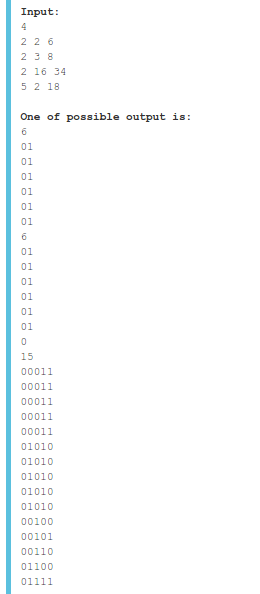
\includegraphics[scale=0.6]{../img/example.png}
\caption{Contoh kasus uji pada GUESSN5}
\label{fig:guessn5_test_case}
\end{figure}

Gambar \ref{fig:guessn5_test_case} adalah contoh empat uji kasus dari permasalahan SPOJ GUESSN5.

\begin{exmp}
Pada uji kasus yang pertama hanya terdapat dua angka. Jika penjawab tidak berbohong, penjawab dapat menjawab pilihan
\begin{align*}
111111 \;\;& 000000\textrm{.}
\end{align*}
Jika penjawab berbohong satu kali, penjawab dapat menjawab 
\begin{align*}
& 111110 & & 111101 & 111011 \\
& 110111 & & 101111 & 011111 \\
& 000001 & & 000010 & 000100 \\
& 001000 & & 010000 & 100000 &\textrm{.}
\end{align*}
Jika penjawab berbohong dua kali, penjawab dapat menjawab
\begin{align*}
& 000011 & & 000101 & 000110 \\
& 001001 & & 001010 & 001100 \\
& 010001 & & 010010 & 010100 \\
& 011000 & & 100001 & 100010 \\
& 100100 & & 101000 & 110000 \\
& 001111 & & 010111 & 011011 \\
& 011101 & & 011110 & 100111 \\
& 101011 & & 101101 & 101110 \\
& 110011 & & 110101 & 110110 \\
& 111001 & & 111010 & 111100 &\textrm{.}
\end{align*}
Penanya memenangkan permainan karena kemungkinan jawaban selain tersebut di atas membuat penjawab akan berbohong tiga kali.
\end{exmp}

\begin{exmp}
Pada uji kasus yang kedua penjawab mencoba memberikan solusi namun jawabannya salah. Penanya dapat menjawab $111000$ yaitu jawaban yang valid karena jumlah bohong tiga kali untuk kedua kemungkinan angka. Pada kasus ini penanya kalah karena penanya membutuhkan query tambahan.
\end{exmp}

\begin{exmp}
Pada uji kasus yang ketiga penanya tidak memberikan solusi.
\end{exmp}

\begin{exmp}
Pada uji kasus yang keempat penanya memberikan query yang lebih sedikit dari jumlah query maksimal yang diperbolehkan. Dari semua kemungkinan jawaban penjawab, pasti hanya ada satu jawaban nilai $x$, jadi penanya memenangkan permainan.
\end{exmp}


\section{Backround of binary code}

Tujuan utama dari teori pengkodean (\textit{coding theory}) adalah bagaimana mengirimkan pesan pada kanal yang mengandung derau (\textit{noisy channel}) \cite{VanLint2016}. Misal jika ada delapan macam kata pesan yang akan dikirim, maka kita merepresentasikan pesan tersebut menjadi bitstring biner dengan panjang 3. Namun jika pesan tersebut dikirm langsung melewati kanal yang mengandung derau, bisa jadi misalkan ada 1 bit akan tertukar, misal $001$ menjadi $011$. Jika terjadi seperti itu, maka sebuah kata dapat tertukar menjadi kata yang lain.

Kita tahu bahwa jika kode biner sepanjang $n$ digunakan untuk membuat $2^n$ bitstring tidak dapat mendeteksi eror. Ide yang paling mungkin adalah pengirim dan penerima menyetujui sebuah metode enkripsi bitstring menjadi bitstring yang lebih panjang dan dapat mendeteksi maksimal sebanyak $e$ error menggunakan kode linear.

Kode linear adalah kode yang paling banyak dipelajari karena struktur aljabar yang mudah dipelajari dibandingkan kode non-linear \cite{Huffman}. Bidang kode linear dapat dinotasikan sebagai $\mathbb{F}_q^n$, yaitu kode memiliki $q$ jenis elemen dan memiliki panjang $n$. Bentuk kode biner adalah $\mathbb{F}_2^n$, memiliki struktur aljabar penjumlahan dan pengurangan sebagai berikut.

\begin{align*}
0 + 0 &= 0 & 0 \cdot 0 &= 0 \\
0 + 1 &= 1 & 0 \cdot 1 &= 0 \\
1 + 0 &= 1 & 1 \cdot 0 &= 0 \\
1 + 1 &= 0 & 1 \cdot 1 &= 1
\end{align*}

\begin{equation} \label{eq:dh}
d_H(\vec{x},\vec{y}) = |\{i \in {1,\ldots,n} \mid x_i \neq y_i\}|
\end{equation}

Jarak Hamming dari bitstring $\vec{x}$ dan $\vec{y}$ dengan panjang $n$ didefinisikan dengan \refeq{eq:dh} \cite{Cicalese2000}. Sebagai contohnya $d_H(0000,1111)= 4$ dan $d_H(00110,00101)= 2$. $d_H(\vec{x},\vec{y})$ juga dapat dikatakan jumlah minimal untuk mentransformasi dari $\vec{x}$ ke $\vec{y}$. Contoh $\vec{x}=00110$ dan $\vec{y}=00101$ memiliki perbedaan pada 2 bit terakhir dengan jarak Hamming 2, dapat dikatakan $\vec{x}+00011 = \vec{y}$.

\begin{equation} \label{eq:wt}
wt(\vec{x}) = |\{i \in {1,\ldots,n} \mid x_i \neq 0\}|
\end{equation}

Bobot dari bitstring $\vec{x}$ didefinisikan dengan $wt(\vec{x})$, yaitu jumlah digit pada $\vec{x}$ yang bukan $0$ seperti pada \refeq{eq:wt}. Sebagai contohnya, $wt(00101) = 2$ dan $wt(11111) = 5$. Jika dihubungkan dengan jarak Hamming, jika $\vec{x}+\vec{e} = \vec{y}$ maka $d_H(\vec{x},\vec{y}) = wt(\vec{x}+\vec{y})$.

Terdapat sebuah sifat pada jarak Hamming yang bernama segitiga pertidaksamaan (\textit{triangle inequality}) \cite{VanLint2016}.
\begin{equation} \label{eq:dh_unequal}
d_H(\vec{x},\vec{y}) \le d_H(\vec{x},\vec{z}) + d_H(\vec{y},\vec{z})
\end{equation}
Dari \refeq{eq:dh_unequal}, misalkan $\vec{z}$ adalah $\vec{0}$ yaitu string biner yang berisi semua $0$, maka didapatkan \refeq{eq:wt_unequal}.
\begin{equation} \label{eq:wt_unequal}
wt(\vec{x}+\vec{y}) \le wt(\vec{x}) + wt(\vec{y})
\end{equation}

Kode biner (\textit{binary code}) adalah sejumlah $M$ bitstring biner dengan panjang masing-masing bitstring adalah $n$ dan jarak Hamming pada masing masing bitstring adalah $d$. Mari kita ambil contoh $M=8$, $n=6$, dan $d=3$ pada Gambar \ref{fig:binarycode683}. Parameter pada kode ini adalah $(6,8,3)_2$, yaitu kode biner yang ditunjukkan pada angka 2, panjang bitstring 6, berisi 8 bitstring, dengan jarak Hamming minimal 3. Bitstring pada kode biner selanjutnya disebut kata kode (\textit{codeword}).

\begin{figure}
\centering
\begin{BVerbatim}
000000  100110
001011  101101
010101  110011
011110  111000
\end{BVerbatim}
\caption{Kode biner $(6,8,3)_2$}
\label{fig:binarycode683}
\end{figure}

Dengan kode biner $(6,8,3)_2$ pada Gambar \ref{fig:binarycode683}, pengirim dan penerima menyepakati hanya kata kode yang akan dikirim dan diterima. Dengan asumsi hanya ada satu bit yang dapat error, pesan error tetap dapat dikembalikan ke bentuk semula. Misal $111100$ menjadi $111000$, $000011$ menjadi $001011$, dan seterusnya. Jarak Hamming antara setiap dua kata kode yang berbeda adalah 3, berarti dari setiap kata kode, terdapat sejumlah bitstring selain kata kode berjarak 1.

\begin{figure}
\centering
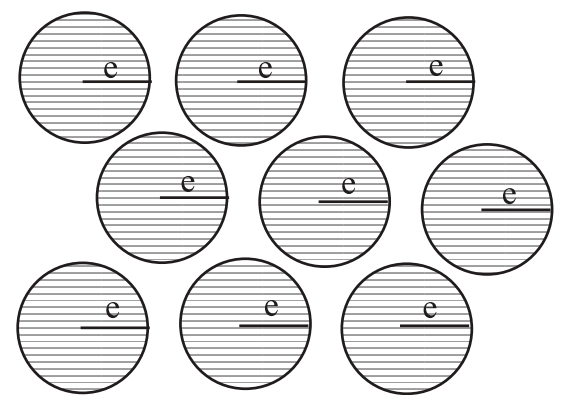
\includegraphics[width=\linewidth]{../img/codewordsball.png}
\caption{Bola codeword yang tidak saling overlap}
\label{fig:codewordsball}
\end{figure}

Notasi umum kode biner adalah $(n,M,d)_2$. Kita bisa asumsikan ada $M$ bola yang tidak saling bersinggungan atau berpotongan, dengan radius bola $e$ seperti pada Gambar \ref{fig:codewordsball}. Jarak antara satu bola dengan bola yang lain adalah minimal $d$, sehingga didapatkan \refeq{eq:de}.
\begin{equation} \label{eq:de}
d = 2e + 1
\end{equation}


\section{Generate binary code with generator matrix}

An $(n,M,d)_2$ binary code can be generated by using linear combination of each row of a generator matrix $[n,m,d]_2$ where $2^m = M$. A Generator matrix $G$ is an $n \times m$ matrix. Now see that binary code $(6,8,3)_2$ in Figure \ref{fig:binarycode683} can be generated using generator matrix $[6,3,3]_2$ in Figure \ref{fig:generator633}. Assume that each row of $[6,3,3]_2$ is $g_1$, $g_2$, and $g_3$, then binary code $(6,8,3)_2$ is the linear combination of all vectors of the form ${\lambda}_1 g_1 + {\lambda}_2 g_2 + {\lambda}_3 g_3$ where $\lambda{_i} \in \mathbb{F}_2^6$.

Now again see a generator matrix $[7,3,4]_2$ in Figure \ref{fig:generator734} can create a perfect binary code $(7,8,4)_2$ code in Figure \ref{fig:binarycode784}. A generator matrix $[n, m, d]_2$ where $n = 2^m - 1$ and each \textbf{column} is a linear combination of $m$ bit binary string except $\vec{0}$ can make a perfect binary code $(n,M,d)_2$ where $d = M/2$. \textbf{\textit{We need a profing or citation..}}

\begin{figure}
\centering
\begin{BVerbatim}
100110
010101
001011
\end{BVerbatim}
\caption{Generator matrix $[6,3,3]_2$}
\label{fig:generator633}
\end{figure}

\begin{figure}
\centering
\begin{BVerbatim}
1001101
0101011
0010111
\end{BVerbatim}
\caption{Generator matrix $[7,3,4]_2$}
\label{fig:generator734}
\end{figure}

\begin{figure}
\centering
\begin{BVerbatim}
0000000  1000111
0011101  1000111
0101011  1000111
0110110  1000111
\end{BVerbatim}
\caption{Perfect binary code $(7,8,4)_2$}
\label{fig:binarycode784}
\end{figure}

Nah masalahnya, jika $d$ yang kita butuhkan kurang dari $M/2$, maka kita harus menggunakan seminimal mungkin $n$ kolom pertama $[M-1,M,M/2]_2$ sehingga menghasilkan $[n,M,d]_2$. Asumsikan kita memiliki fungsi $\aleph(d)$ adalah berapa kolom pada generator matrix yang akan menghasilkan kode biner dengan minimal jarak Hamming $d$. Hal yang pasti adalah $\aleph(M/2) = M-1$ dan $\aleph(1) = {log}_2(m)$ (need proving). Worst case adalah $\aleph(d)=M/2 + d - 1$. Best case adalah karena ada $M-1$ kolom untuk $0 \leq d \leq M/2$, maka $\aleph(d) = d/2$ (sepertinya tidak mungkin). Nah problem kita adalah bagaimana mengurutkan kolom pada generator matrix sehingga $\aleph(d)$ sesempurna mungkin, atau bisa dikatakan $\aleph(d) - \aleph(d-1) \approx 2$.

% Assume that $g_i$ is row of $G$. Then we iterate each $g_i$ to make new query until Hamming distance reaches what we need. If we need more than $M/2$ Hamming distance, repeat.

% \begin{enumerate}
%   \item A $g$ is a binary string $\mathbb{F}_2^m$
% \end{enumerate}


\section{Solusi permainan Ulam non-interaktif}

Diberikan sebuah matriks $L$ berukuran $n \times M$ berisi $n$. Kumpulan query ini dinotasikan dengan $L = \{\vec{q_1},\vec{q_2},\ldots,\vec{q_n}\}$ dimana $\vec{q_i} = \{s_1,s_2,\ldots,s_M\}$. Himpunan nilai $s_i$ yang mungkin adalah $s_i \in \{0,1\}$. Diberikan sebuah vektor $\vec{z} \in \{z_1,z_2,\ldots,z_n\}$ dimana $z_i \in \{0,1\}$ berisi jawaban dari seluruh query secara berurutan, $z_i$ adalah jawaban dari $\vec{q_i}$, dimana $0$ berarti 'tidak' dan $1$ berarti 'ya'. Karena jika jawaban $0$ berarti query harus ditambah dengan 1 dan jika jawaban $1$ berarti query ditambah dengan 0 (diabaikan), maka kita memiliki $\vec{z'}$ yaitu inverse dari $\vec{z}$. 

Matriks $L'$ berukuran $M \times n$ adalah hasil transpose dari matriks $L$. Tambahkan seluruh baris pada $L'$ dengan $z'$. Maka jawaban dari permainan Ulam non-interaktif adalah index dari baris $r$ pada $L'$ yang memiliki bobot $wt(\vec{x_r}) > n-e$.

Penanya memenangkan permainan jika $L'$ memiliki paling banyak satu row dengan $wt(\vec{x}) \ge n-e$. Jika hanya ada satu row, maka row tersebut adalah jawaban permainan. Jika tidak ada satu row pun yang memenuhi, penanya tetap memenangkan permainan karena penjawab melakukan kecurangan, melakukan bohong untuk semua angka lebih dari batas yang ditetapkan.

Untuk meyakinkan bahwa setelah seluruh jawaban $\vec{z}$ diberikan dan diaplikasikan ke matrix $L$ dan tidak pasti hanya ada 1 baris yang memiliki nilai $1$ antara $n-e \le wt(\vec{x_r}) \le n$, adalah dengan memastikan bahwa jarak Hamming setiap row yang berbeda pada $L'$ adalah minimal $d$.

\begin{lemma}
Diketahui integer $n$, $M$, dan $d$. Jika $L'$ adalah kode biner $(n,M,d)_2$ yang valid, maka pasti hanya ada paling banyak satu codeword $\vec{c}$ yang memiliki $0 \le wt(\vec{c}) \le e$.
\end{lemma}

\begin{proof}
Jika ada codeword $c$ dimana $0 \le wt(c) \le e$ maka $wt(\vec{x}) > e$ dimana $\vec{x} \neq c$. Pembuktian dapat dibuktikan dengan dua kasus.\\

1) Jika $wt(\vec{c}) = 0$ maka
\begin{align*}
d_H(\vec{c},\vec{x}) &\ge d \mid \vec{c} \neq \vec{x} , \vec{x} \in L' \\
wt(\vec{c} + \vec{x}) &\ge d \\
wt(\vec{x}) &\ge d \label{eq:proofd} \stepcounter{equation} \tag{\theequation}
\end{align*}
Sebelumnya telah disebutkan hubungan $d$ dan $e$ pada \refeq{eq:de}. Persamaan tersebut dapat diturunkan menjadi
\begin{equation} \label{eq:dge}
d > e
\end{equation}
Dengan memasukkan \refeq{eq:dge} ke \refeq{eq:proofd}, maka didapatkan
\begin{equation*}
wt(\vec{x}) > e
\end{equation*}

2) Jika $wt(\vec{c}) = e$ maka
\begin{align*}
d_H(\vec{c},\vec{x}) &\ge d \mid \vec{c} \neq \vec{x} , \vec{x} \in L' \\
wt(\vec{c}+\vec{x}) &\ge d \\
wt(\vec{c}) + wt(\vec{x}) \ge wt(\vec{c}+\vec{x}) &\ge d \\
wt(\vec{c}) + wt(\vec{x}) &\ge d \\
e + wt(\vec{x}) &\ge d \\
\intertext{Masukkan \refeq{eq:de} untuk mensubstitusi $d$}\\
wt(\vec{x}) &\ge 2e+1-e \\
&\ge e+1\\
wt(\vec{x}) &> e
\end{align*}
Jadi jika ada codeword $c$ dimana $0 \le wt(c) \le e$ maka $wt(\vec{x}) > e$ dimana $\vec{x} \neq c$.
\end{proof}

Dari pembuktian diatas, dapat disimpulkan bahwa untuk menyelesaikan permainan pencarian Ulam non-interaktif dengan batas pencarian $M$ dan maksimal kebohongan $e$, transpose dari $n$ query yang dibuat harus membentuk kode biner $(n,M,d)_2$.

\begin{lemma}
Diketahui integer $n$, $M$, dan $d$. Jika $L'$ adalah kode biner $(n,M,d)_2$ yang valid, maka jika setiap codeword $\vec{c}$ pada $L'$ ditambah dengan $\vec{z} \mid \vec{z} \in \mathbb{F}_2^n$ maka hasilnya akan tetap menjadi kode biner $(n,M,d)_2$ yang valid.  
\end{lemma}

\begin{proof}
Jika $d_H(\vec{x_i},\vec{y_j}) \ge d \mid \vec{x_i},\vec{y_j} \in L'$ maka
\begin{align*}
d_H(\vec{x_i}+\vec{z},\vec{y_j}+\vec{z}) &\ge d \\
wt(\vec{x_i}+\vec{y_j}+\vec{z}+\vec{z}) &\ge d \\
wt(\vec{x_i}+\vec{y_j}) &\ge d \\
d_H(\vec{x_i},\vec{y_j}) &\ge d \\
\end{align*}
Jadi jika $d_H(\vec{x_i},\vec{y_j}) \ge d$ maka $d_H(\vec{x_i}+\vec{z},\vec{y_j}+\vec{z}) \ge d$.
\end{proof}


\bibliography{holy}

\end{document}
